%% abtex2-modelo-trabalho-academico.tex, laurocesar
%% Copyright 2012-2015 by abnTeX2 group at http://www.abntex.net.br/
%%
%% This work may be distributed and/or modified under the
%% conditions of the LaTeX Project Public License, either version 1.3
%% of this license or (at your option) any later version.
%% The latest version of this license is in
%%	http://www.latex-project.org/lppl.txt
%% and version 1.3 or later is part of all distributions of LaTeX
%% version 2005/12/01 or later.
%%
%% This work has the LPPL maintenance status `maintained'.
%%
%% The Current Maintainer of this work is the abnTeX2 team, led
%% by Lauro César Araujo. Further information are available on
%% http://www.abntex.net.br/
%%
%% This work consists of the files abntex2-modelo-trabalho-academico.tex,
%% abntex2-modelo-include-comandos and abntex2-modelo-references.bib
%%

% ------------------------------------------------------------------------
% ------------------------------------------------------------------------
% abnTeX2: Modelo de Trabalho Academico (tese de doutorado, dissertacao de
% mestrado e trabalhos monograficos em geral) em conformidade com
% ABNT NBR 14724:2011: Informacao e documentacao - Trabalhos academicos -
% Apresentacao
% ------------------------------------------------------------------------
% ------------------------------------------------------------------------

\documentclass[
	% -- opções da classe memoir --
	12pt,				% tamanho da fonte
	openright,			% capítulos começam em pág ímpar (insere página vazia caso preciso)
	oneside,			% para impressão em verso e anverso. Oposto a oneside
	a4paper,			% tamanho do papel.
	% -- opções da classe abntex2 --
	chapter=TITLE,		% títulos de capítulos convertidos em letras maiúsculas
	%section=TITLE,		% títulos de seções convertidos em letras maiúsculas
	%subsection=TITLE,	% títulos de subseções convertidos em letras maiúsculas
	%subsubsection=TITLE,% títulos de subsubseções convertidos em letras maiúsculas
	% -- opções do pacote babel --
	english,			% idioma adicional para hifenização
	french,				% idioma adicional para hifenização
	spanish,			% idioma adicional para hifenização
	brazil				% o último idioma é o principal do documento
	]{abntex2}

% Pacotes básicos
\usepackage{helvet}			% Usa a fonte Latin Modern - Mudei para Helvetica
\usepackage[T1]{fontenc}		% Selecao de codigos de fonte.
\usepackage[utf8]{inputenc}	% Codificacao do documento (conversão automática dos acentos)
\usepackage{lastpage}		% Usado pela Ficha catalográfica
\usepackage{indentfirst}		% Indenta o primeiro parágrafo de cada seção.
\usepackage{color}			% Controle das cores
\usepackage{graphicx}		% Inclusão de gráficos
\usepackage{microtype} 		% para melhorias de justificação


% Pacotes adicionais, usados apenas no âmbito do Modelo Canônico do abnteX2
\usepackage{lipsum}				% para geração de dummy text
\usepackage{customizacoes} 		% customizações feitas pelo autor

% Pacotes de citações
\usepackage[brazilian,hyperpageref]{backref}	% Paginas com as citações na bibl
\usepackage[alf]{abntex2cite}				% Citações padrão ABNT


% CONFIGURAÇÕES DE PACOTES
% Configurações do pacote backref
% Usado sem a opção hyperpageref de backref
\renewcommand{\backrefpagesname}{ }
% Texto padrão antes do número das páginas
\renewcommand{\backref}{\ABNTEXchapterfont}
% Define os textos da citação
\renewcommand*{\backrefalt}[4]{
	\ifcase #1 %
		%
	\or
		%
	\else
		%
	\fi}%

% Informações de dados para CAPA e FOLHA DE ROSTO
\titulo{Habilitando um Prédio a Localizar Contextualmente Dispositivos utilizando Redes Sem Fio}
\autor{Luís Henrique Puhl de Souza}
\local{Bauru}
\data{2016}
\orientador{Prof. Dr. Eduardo Martins Morgado}

\instituicao{%
  Universidade Estadual Paulista ``Júlio de Mesquita Filho''
  %\par
  Faculdade de Ciências - Campus Bauru
  %\par
  Departamento de Computação
}
\tipotrabalho{Monografia (Trabalho de Conclusão de Curso)}
% O preambulo deve conter o tipo do trabalho, o objetivo,
% o nome da instituição e a área de concentração
\preambulo{ Projeto de Trabalho de Conclusão de Curso de Bacharelado em Ciência
da Computação da Universidade Estadual Paulista ``Júlio de Mesquita Filho'',
Faculdade de Ciências, Campus Bauru }

% Configurações de projeto
\newif\iffinal
\finalfalse % define se é um arquivo final, se for não for retira umas partes.

\newif\ifabstract
\abstractfalse % define se mostra o abstract em inglês ou não.

% Configurações de aparência do PDF final
% alterando o aspecto da cor azul
\definecolor{blue}{RGB}{0,0,0}

% informações do PDF
\makeatletter
\hypersetup{
	  	%pagebackref=true,
		pdftitle={\@title},
		pdfauthor={\@author},
	 	pdfsubject={\imprimirpreambulo},
		 pdfcreator={LaTeX with abnTeX2},
		pdfkeywords={beacon}{raspberry pi}{internet das coisas}{abntex2}{trabalho acadêmico},
		colorlinks=true,		 		% false: boxed links; true: colored links
	 	linkcolor=blue,			 	% color of internal links
	 	citecolor=blue,		  		% color of links to bibliography
	 	filecolor=magenta,				% color of file links
		urlcolor=blue,
		bookmarksdepth=4
}
\makeatother

% Espaçamentos entre linhas e parágrafos
% O tamanho do parágrafo é dado por:
\setlength{\parindent}{1.3cm}

% Controle do espaçamento entre um parágrafo e outro:
\setlength{\parskip}{0.2cm}  % tente também \onelineskip

% compila o indice
\makeindex

% Início do documento
\begin{document}

% Seleciona o idioma do documento (conforme pacotes do babel)
%\selectlanguage{english}
\selectlanguage{brazil}

% Retira espaço extra obsoleto entre as frases.
\frenchspacing

% ----------------------------------------------------------
% ELEMENTOS PRÉ-TEXTUAIS
% ----------------------------------------------------------
\pretextual

\ABNTEXchapterfont {

% Capa
\imprimircapa

% Folha de rosto
% (o * indica que haverá a ficha bibliográfica)
%\imprimirfolhaderosto

% Inserir a ficha bibliografica

% Isto é um exemplo de Ficha Catalográfica, ou ``Dados internacionais de
% catalogação-na-publicação''. Você pode utilizar este modelo como referência.
% Porém, provavelmente a biblioteca da sua universidade lhe fornecerá um PDF
% com a ficha catalográfica definitiva após a defesa do trabalho. Quando estiver
% com o documento, salve-o como PDF no diretório do seu projeto e substitua todo
% o conteúdo de implementação deste arquivo pelo comando abaixo:
%
% \begin{fichacatalografica}
%	  \includepdf{fig_ficha_catalografica.pdf}
% \end{fichacatalografica}

\iffinal
  \begin{fichacatalografica}
	\sffamily
	\vspace*{\fill}					% Posição vertical
	\begin{center}					% Minipage Centralizado
	\fbox{\begin{minipage}[c][8cm]{13.5cm}		% Largura
	\small
	\imprimirautor
	%Sobrenome, Nome do autor

	\hspace{0.5cm} \imprimirtitulo  / \imprimirautor. --
	\imprimirlocal, \imprimirdata-

	\hspace{0.5cm} \pageref{LastPage} p. : il. (algumas color.) ; 30 cm.\\

	\hspace{0.5cm} \imprimirorientadorRotulo~\imprimirorientador\\

	\hspace{0.5cm}
	\parbox[t]{\textwidth}{\imprimirtipotrabalho~--~\\ \imprimirinstituicao,
	\imprimirdata.}\\

	\hspace{0.5cm}
		2. Internet das Coisas.
		I. \imprimirorientador.
		II. Universidade Estadual Paulista ``Júlio de Mesquita Filho''.
		III. Faculdade de Ciências.
		IV. Título
	\end{minipage}}
	\end{center}
  \end{fichacatalografica}
\fi

% INSERIR ERRATA
%\begin{errata}
%Elemento opcional da \citeonline[4.2.1.2]{NBR14724:2011}. Exemplo:

%\vspace{\onelineskip}

%FERRIGNO, C. R. A. \textbf{Tratamento de neoplasias ósseas apendiculares com
%reimplantação de enxerto ósseo autólogo autoclavado associado ao plasma
%rico em plaquetas}: estudo crítico na cirurgia de preservação de membro em
%cães. 2011. 128 f. Tese (Livre-Docência) - Faculdade de Medicina Veterinária e
%Zootecnia, Universidade de São Paulo, São Paulo, 2011.

%\begin{table}[htb]
%\center
%\footnotesize
%\begin{tabular}{|p{1.4cm}|p{1cm}|p{3cm}|p{3cm}|}
%  \hline
%	\textbf{Folha} & \textbf{Linha}  & \textbf{Onde se lê}  & \textbf{Leia-se}  \\
%	 \hline
%	 1 & 10 & auto-conclavo & autoconclavo\\
%	\hline
%\end{tabular}
%\end{table}

%\end{errata}


% INSERIR FOLHA DE APROVAÇÃO
% Isto é um exemplo de Folha de aprovação, elemento obrigatório da NBR
% 14724/2011 (seção 4.2.1.3). Você pode utilizar este modelo até a aprovação
% do trabalho. Após isso, substitua todo o conteúdo deste arquivo por uma
% imagem da página assinada pela banca com o comando abaixo:
%
% \includepdf{folhadeaprovacao_final.pdf}
%
\begin{folhadeaprovacao}
  \ABNTEXchapterfont {

	 \begin{center}

		{\ImprimirAutor}

		\vspace*{\fill}\vspace*{\fill}

		\begin{center}
		  \bfseries\large\ImprimirTitulo
		\end{center}

		\vspace*{\fill}

		\hspace{.45\textwidth}
		\begin{minipage}{.5\textwidth}
			 \imprimirpreambulo
		\end{minipage}%
		\vspace*{\fill}
	  \end{center}

	  %Trabalho aprovado. \imprimirlocal, 24 de novembro de 2012:

	  %\assinatura{\textbf{\imprimirorientador} \\ Orientador}
	  %\assinatura{\textbf{\imprimircoorientador} \\ Coorientador}
	  %\assinatura{\textbf{Professor} \\ Convidado 1}
	  %\assinatura{\textbf{Professor} \\ Convidado 2}
	  %\assinatura{\textbf{Professor} \\ Convidado 3}
	  %\assinatura{\textbf{Professor} \\ Convidado 4}
		\vspace*{0.5cm}
		\hspace{.5\textwidth}
	  \begin{center}
		 \ImprimirLocal \\ \imprimirdata
	  \end{center}
  }
\end{folhadeaprovacao}

% DEDICATÓRIA
\iffinal
  \begin{dedicatoria}
	\vspace*{\fill}
	\centering
	\noindent
	\textit{} \vspace*{\fill}
  \end{dedicatoria}
\fi

% AGRADECIMENTOS
\iffinal
	\begin{agradecimentos}
	\end{agradecimentos}
\fi

% EPÍGRAFE
\iffinal
  \begin{epigrafe}
	 \vspace*{\fill}
	\begin{flushright}
		\textit{}
	\end{flushright}
  \end{epigrafe}
\fi

% RESUMOS
\ifabstract
% RESUMO EM PORTUGUÊS
\setlength{\absparsep}{18pt} % ajusta o espaçamento dos parágrafos do resumo
\begin{resumo}
	\ABNTEXchapterfont {
		\textbf{Palavras-chave}: IoT. Internet das Coisas. GPS de interiores. Posicionamento Contextual.
	}
\end{resumo}

% RESUMO EM INGLÊS
\begin{resumo}[Abstract]
	\begin{otherlanguage*}{english}
		This is the english abstract.
		\vspace{\onelineskip}
		\noindent
		\textbf{Keywords}: IoT. Indoor GPS. Contextual Positioning.
	 \end{otherlanguage*}
\end{resumo}
\fi

% INSERIR LISTA DE ILUSTRAÇÕES
\iffinal
  \pdfbookmark[0]{\listfigurename}{lof}
  \listoffigures*
  \cleardoublepage
\fi

% INSERIR LISTA DE TABELAS
\iffinal
  \pdfbookmark[0]{\listtablename}{lot}
  \listoftables*
  \cleardoublepage
\fi

% INSERIR LISTA DE ABREVIATURAS E SIGLAS
\iffinal
  \begin{siglas}
	 \item[ANN] \textit{Artificial Neural Networks}
  \end{siglas}
\fi

% INSERIR LISTA DE SÍMBOLOS
\iffinal
  \begin{simbolos}
	 \item[$ \Gamma $] Letra grega Gama
	 \item[$ \Lambda $] Lambda
	 \item[$ \zeta $] Letra grega minúscula zeta
	 \item[$ \in $] Pertence
  \end{simbolos}
\fi

% INSERIR O SUMARIO
\pdfbookmark[0]{\contentsname}{toc}
\tableofcontents*
\cleardoublepage


% ------------------------------------------------------------------------------
% ELEMENTOS TEXTUAIS
% ------------------------------------------------------------------------------
\textual

\chapter[Introdução]{Introdução}
%\addcontentsline{toc}{chapter}{Introdução}

\textbf{\underline{Contexto}}

\underline{IoT como foco}

Recentemente IoT (\textit{Internet of Things} - Internet das Coisas) vem tomando
o foco das atenções de empresas e entusiastas de IT (\textit{Information
Tecnology} - Tecnologia da Informação) \cite{DzoneIoT:2015} a tal ponto que as
empresas líderes do segmento já incluem IoT como uma de suas áreas de atuação
\cite{Ibm2016} \cite{ARM-mbed} \cite{Microsoft2016} \cite{Intel2016}
\cite{Oracle2016} \cite{Google2016} \cite{AmazonIoT2016}.

Todo este movimento no mercado é justificado pelo baixo custo dos pequenos
dispositivos computacionais \cite{RpiZeroLaunch} \cite{Esp8266.net} e grandes
serviços na nuvem \cite{Kaufmann2015} \cite{Amazon2016}. Este baixo custo
possibilita a computação ubíqua descrita por Weiser em 1991 e 1992
\cite{Weiser1999} que é entendida pelos autores como ``computação virtualmente
onipresente''. Também para os autores, esta virtual onipresença é base e
consequência para a IoT sendo esta a realizadora da computação ubíqua.

Uma vez contextualizado o mercado e a oportunidade de implementação da
computação ubíqua, percebemos a necessidade de dar aos elementos cotidianos
(coisas) a capacidade info-computacional, tornando-os sensores e atuadores
conectados, unicamente identificáveis e acessíveis através da rede mundial
(internet) \cite{Lemos2013} \cite{Kranenburg2012}.

\underline{Numero de dispositivos}

É esperado que uma quantia total de 6,4 bilhões de dispositivos conectados
exista até o final de 2016 \cite{GARTNER2015} e entre 26 bilhões
\cite{GARTNER2014}  e 50 bilhões até 2020 com até 250 novas coisas conectando-se
por segundo \cite{CiscoBlog2013}.


\textbf{\underline{Problema}}
\underline{Grande quantidade de dispositivos}

Tamanha quantidade de dispositivos conectados pouco acrescenta na vida diária se
humanos ou coisas não puderem simplesmente se encontrar, tanto em ambiente real
quanto virtual é necessário o contato entre as partes para a existencia de uma
interação.

Mais ainda, para melhor funcionamento de aplicações, em especial o oferecimento
de conteúdo específico para cada usuário, é necessário contextualizar e o
primeiro passo da contextualização é a conciência da localização.

\underline{Exemplo da perda de aparelhos no predio (zebra) (ou outro exemplo)}

Um exeplo da necessidade de localização de dispositivos dentro de um prédio
seria um profissional saber onde está o dispositivo em seu local de trabalho,
seja ele um vendedor e seu tablet para demostrar um produto fora de estoque em
uma loja ou um médico e um desfibrilador.


% \underline{Nota do autor: Introduza o problema de localizar e contextualizar
% cada dispositivo.}


% Entendemos que devido a natureza física e info-computacional das coisas
% conectadas tanto sua localização e identificação na rede de comunicação
% (endereço lógico, de internet, IPv6 ou URI) quanto sua localização e
% identificação física (posicionamento global e relativo, identidade física) são
% de igual importância.


% Porém para os autores apenas a localização lógica foi bem resolvida, documentada
% e padronizada pela ciência da computação pois sistemas de localização físicos,
% apesar de existirem e funcionarem perfeitamente no dia-a-dia especialmente em
% ambientes abertos, não são tão onipresentes quanto os lógicos nem trazem
% contextualização de maneira tão simples.

% Para exemplificar esta visão dos autores faremos uma comparação entre uma
% localização no formato oferecido por um sistema de posicionamento global (GPS)
% como o trio Latitude, Longitude e elevação com um endereço lógico na internet, o
% endereço IPv6. Nesta camada é possível comparar o nível de abrangência dos dois
% protocolos da mesma maneira que comparamos números.


% Porém as similaridades tornam-se estreitas no próximo nível de abstração
% considerando para endereço lógico uma URI (\textit{Uniform Resource Identifier})
% com um DNS (\textit{Domain Name System}) propriamente aplicado quando comparamos
% a um endereço físico contendo País, Região, Cidade, Bairro, Rua, Número de rua,
% número de repartição (apartamento, casa), identificação do cômodo (unitário,
% atômico nesta especificação) e finalmente uma posição relativa dentro deste
% cômodo cuja complexidade não diminui mesmo quando levamos em conta técnicas de
% endereçamento como ZIP e CEP.


% Para diminuição desta complexidade podemos abordar o problema fora da teoria de
% informação com um ponto de vista geométrico utilizando uma posição GPS comum até
% a fase de repartição (até onde GPS via satélite é eficiente) e dentro da
% repartição (fora de alcance dos satélites) utilizar uma nova coordenada de
% Direção e Distância a partir de um ponto fixo único desta repartição.



\underline{Soluções corelatas}

\underline{Nota do autor: Introduza os meios existentes de localização (marcelo).}

% GPS não funciona bem indoor, existem 2 tipos de indoor

Os tradicionais sistemas de GPS (Global Positioning System) utilizam a
técnica de auto posicionamento para calcular sua posição no globo terrestre baseado
nos sinais recebidos de 24 satélites posicionados na órbita terrestre com 20.200
kilômetros de distância entre cada um \cite{Djuknic2001}.


Entretanto, a força do sinal GPS não é suficiente para penetrar a maioria dos
prédios. A reflexão do sinal muitas vezes permite a leitura em ambientes
fechados, porém o cálculo da posição não será confiável
\cite{Dartmouth2000}. Portanto, são necessárias soluções diferentes para
se criar um sistema de geoposicionamento que funcione em ambientes fechados.


\textbf{\underline{Revisado até aqui}}

\textbf{\underline{Nossa solução}}

\underline{Ambiente conciente}

\underline{Nota do autor: Introduza nossa solução.}



Por exemplo, utilizando uma série de sensores wi-fi posicionados em pontos
fixos dentro de um prédio, com a triangulação do sinal é possível calcular a posição
de dispositivos conectados à rede wi-fi [BLECKY, 2016].



Para oferecer uma posição confiável, é necessário que estes sensores
coletem e transmitam a força do sinal wi-fi em cada dispositivo com uma alta
frequência.


\textbf{\underline{Justificativa }}\\


\underline{Economia em cada aparelho}\\

Escolhemos o sistema de antenas sensoras e dispositivos transmissores ao invés
do contrario (explicar com o detalhes o pq da escolha e falar o que é contrário)
para economia de harware no sentido de menos hardware em cada dispositivo e
levando em conta  a quantidade prevista de em média 5 dispositivos conectados
por pessoa e de que, com este sistema, estes dispositivos não precisariam de
sensores para localizar-se além de informações mais completas para o prédio.

\underline{Funcionamento por prédio} \\
 -> \underline{uma vez instalado qualquer quantidade de
devices é recebida, facil gerencia dentro do predio}\\
 -> \underline {beneficios para o admin do predio}\\


Utilizando como exemplo o prédio do Laboratório de Tecnologia da
Informação Aplicada (LTIA) da Faculdade de Ciências da Unesp de Bauru, em um dia
comum, é observado uma média de 30 dispositivos conectados à rede wi-fi.

Considerando um sensor que a cada 30 segundos colete 1 kB de dados de cada
dispositivo, por mês, seriam coletados mais de 2 GB de dados. Portanto, para garantir
um sistema escalável, é necessário a utilização de técnicas de Big Data para
armazenar e manipular esses dados.
O melhor modo de se definir Big Data ainda é discutido por pesquisadores,
mas uma definição simples é a de que “se é necessário se preocupar com o tamanho
dos dados, então é Big Data.” (ESPOSITO, 2015, tradução nossa)


\chapter{Problema}
A grande quantidade de dispositivos traz o desafio de localizá-los contextualmente, tanto para que o dispositivo tome ciência de sua posição em um contexto além de sua posição global em suas tomadas de decisão e para que outros (sistemas, pessoas e coisas) saibam a localização de qualquer dispositivo ao qual têm interesse de interagir.

Mesmo com a grande quantidade de dispositivos já conectados são poucos os documentos descrevendo boas práticas para concepção, construção e manutenção de aplicações IoT, especialmente sobre os cuidados tomados quanto a segurança e análise de custos para a implementação e manutenção.

Além disso, a falta de referências neste sentido é agravada quando considera-se implementação no interior do estado de São Paulo visto que poucas são as organizações atualizadas neste tema levando a uma falta enorme de conteúdo escrito na linguagem local além de serviços e produtos disponíveis para construção de uma plataforma completa e competitiva nesta região.

\chapter{Justificativa}

\underline{Nota do parecerista: Reescrever}

Na visão dos autores, promover o desenvolvimento local através de trabalhos exemplo, treinamentos ou manuais é fundamental para a equiparação dos desenvolvedores locais com as tecnologias e tendencias de mercado então justificamos sua execução para que outras organizações possam encontrar novos caminhos.

\chapter{Objetivos}

\section{Objetivos Gerais}

\underline{Nota do parecerista: Este não é o objetivo do TCC do Marcelo Augusto Cordeiro??}

Considerando características locais, propõem-se a construção de uma aplicação para localizar contextualmente dispositivos dentro de um prédio piloto e avaliar sua precisão.

Além desta aplicação, é objetivo definir o custo do projeto piloto incluindo esforço de pesquisa assim como definir um custo para replicação deste localizador contextual em outros prédios.

\section{Objetivos Específicos}

\begin{alineas}
	\item Estabelecer o estado da arte sobre a desenvolvimento de aplicações IoT;
	\item Identificar desafios locais para o desenvolvimento;
	\item Identificar provedores de serviços, dispositivos e ferramentas para o desenvolvimento;
	\item Construir um protótipo de sala conectada virtualmente que identifique os dispositivos conectados a rede que existem dentro nela através de conexões sem fio;
	\item Estimar o custo total do projeto piloto incluindo esforço de pesquisa;
	\item Estimar o custo de replicação da aplicação em outros prédios.
\end{alineas}

\underline{Nota do parecerista: Na proposta do Marcelo, foi informado que o Luís Henrique ficará responsável por todos os sensores, o que inclui sua construção, posicionamento, configuração e programação dos gateways.}

\chapter{Método de Pesquisa}

Utilizaremos prototipagem ágil semelhante ao desenvolvimento de um produto utilizando a metodologia \textit{Scrum} \cite{James2016}, executando iterações de uma semana onde a cada iteração uma nova versão melhorada do produto completo (hardware, software, documentação e resultados) será entregue.

Dentro de cada iteração as camadas da aplicação IoT serão escolhidas, implementadas, justificadas e avaliadas sendo todo processo documentado. Como resultado de cada iteração será gerado um relatório das mudanças a partir da iteração anterior.

\begin{figure}[htb]
	\caption{\label{fig:projeto}Modelo das camadas }
	\begin{center}
		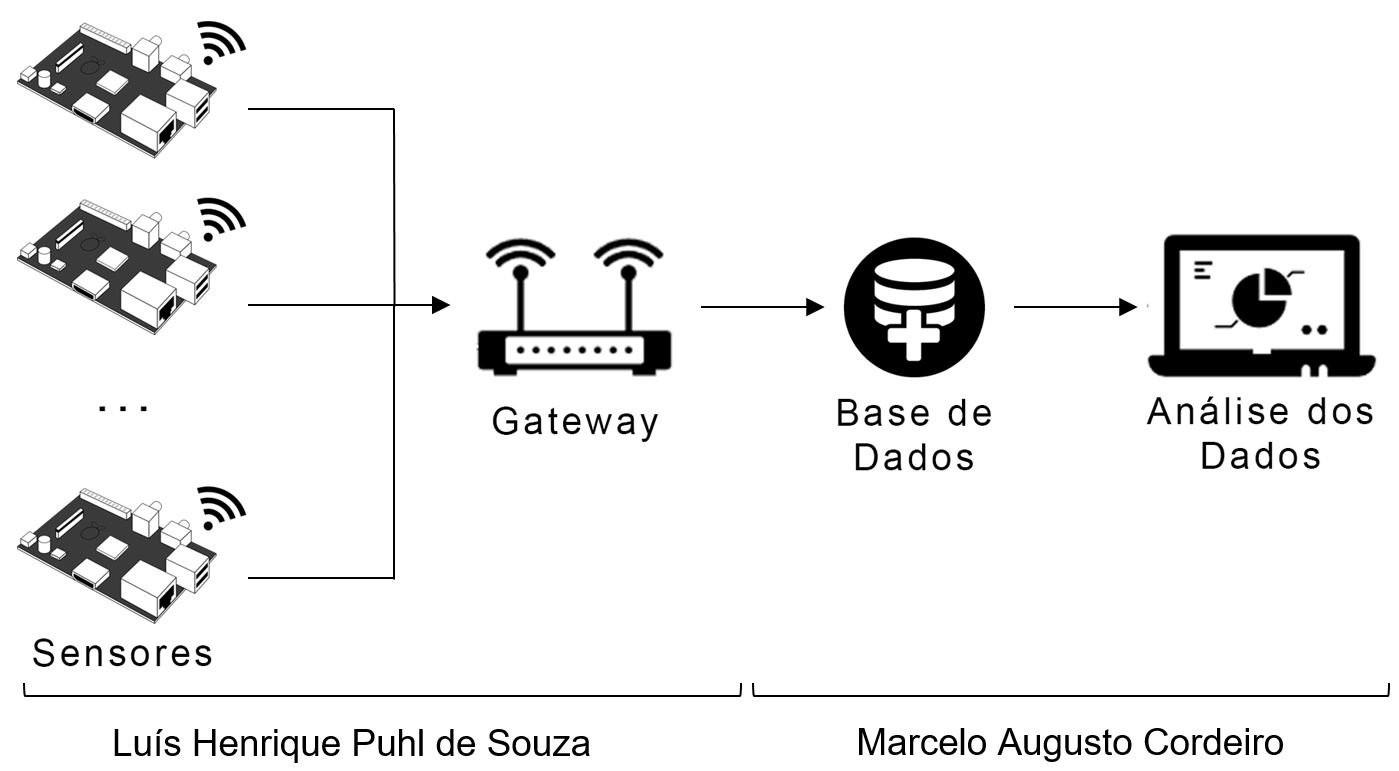
\includegraphics[width=1\textwidth]{img/projeto.JPG}
	\end{center}
	\legend{Fonte: Marcelo Augusto Cordeiro}
\end{figure}

A Figura \ref{fig:projeto} apresenta a arquitetura simplificada de uma aplicação IoT. Esta será modificada a cada iteração do projeto especialmente as camadas de sensores, \textit{gateway} e base de dados.

\underline{Nota do parecerista: Reescrever a metodologia....descrever detalhadamente as atividades que deverão ser desenvolvidas}


% Fundamentação Teórica
%\chapter{Fundamentação Teórica}

%Precisa?


% Cronograma
\chapter{Cronograma}


Devido a natureza ágil e iterativa da metodologia, o cronograma será dividido em apenas três partes: Levantamento Bibliográfico Inicial, Desenvolvimento Iterativo e Revisão Final. Estas partes serão distribuídas conforme a Tabela~\ref{table:cronograma}.

\begin{table}[htb]
\IBGEtab{%
\ABNTEXchapterfont {
  \caption{Cronograma de Atividades Propostas}%
  \label{table:cronograma}
}
}{%
  \begin{tabular}{cccccccccc}
  \toprule
	Atividade							&	Fev	&	Mar	&	Abr	&	Mai	&	Jun	&	Jul	&	Ago	&	Set	&	Out \\
  \midrule \midrule
	Levantamento Bibliográfico Inicial	&	X	&	X	&	 	&	 	&	 	&	 	&	 	&	 	&	  \\
  \midrule
  Desenvolvimento Iterativo				&	 	&	X	&	X	&	X	&	X	&	X	&	X	&	X	&	  \\
  \midrule
  Revisão Final							&	 	&	 	&	 	&	 	&	 	&	 	&	 	&	X	&	X \\
  \bottomrule
\end{tabular}%
}{%
  \fonte{Produzido pelo autor.}%
  }
\end{table}

\underline{Nota do parecerista: A atividade ``Desenvolvimento Iterativo'' deve ser dividida em sub-atividades...}



% Conclusão
%\chapter{Conclusão}

%\lipsum[1]



% ----------------------------------------------------------------------------------------------------------------------------------






% ----------------------------------------------------------
% ELEMENTOS PÓS-TEXTUAIS
% ----------------------------------------------------------

% ----------------------------------------------------------

% ----------------------------------------------------------
% Referências bibliográficas
% ----------------------------------------------------------
\bibliography{referencias}

}
\end{document}
